% =====================================================================
%  wp_meas: informal ↔ formal  —  2 slides
%
%  Slide 1: the proof itself   — WPMeas.lean (271) + WPUnifHelpers.lean (115)
%  Slide 2: the infrastructure — BI (224) + Assertion (176) + Appl (211)
%                                + Std (326) + MeasureProduct (132)
%                                + KRM (538) + MeasureOnSpace (911)
%
%  All 9 files = 2904 lines required by wp_meas, nothing else.
% =====================================================================

\definecolor{colorFP}{HTML}{1565C0}
\definecolor{colorWit}{HTML}{E65100}
\definecolor{colorMeas}{HTML}{2E7D32}
\definecolor{colorPCM}{HTML}{6A1B9A}
\definecolor{colorBind}{HTML}{B71C1C}
\definecolor{colorPost}{HTML}{00695C}

\newcommand{\WPMeas}{../Bppl/Lilac/ProofRules/WPMeas.lean}
\newcommand{\MeasProd}{../Bppl/Lilac/ProofRules/MeasureProduct.lean}
\newcommand{\WPUnif}{../Bppl/Lilac/ProofRules/WPUnifHelpers.lean}

% Zero-gap inputminted block
\newcommand{\cb}[4]{%  #1=bgcolor  #2=first  #3=last  #4=file
  \vspace{-1pt}%
  \inputminted[fontsize=\fontsize{2pt}{2.2pt},bgcolor=#1,
    firstline=#2,lastline=#3,breaklines=false,
    tabsize=2,framesep=0pt,framerule=0pt]{lean4}{#4}%
  \vspace{-1pt}%
}

% Shared: left column with informal proof overlays
% Image: 760x457px (cropped), fractions = y_new / 457
% Coloured bands cover every line of the paragraph — no white gaps.
\newcommand{\informalProof}{%
  \vspace{-4pt}
  \begin{tikzpicture}
    \node[anchor=north west, inner sep=0pt] (img) at (0,0)
      {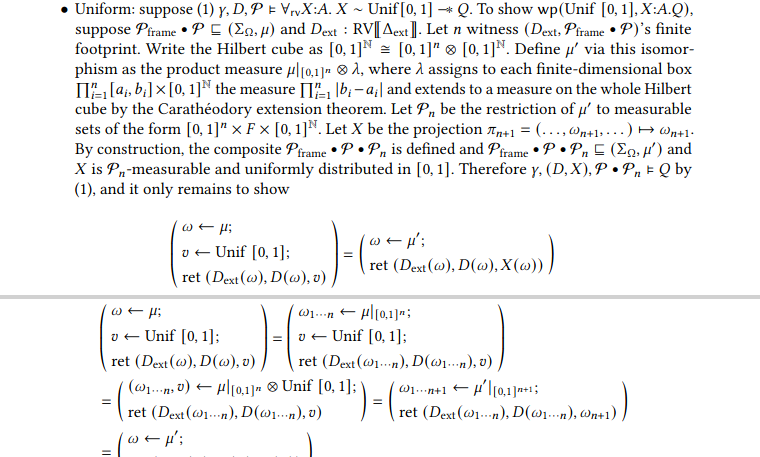
\includegraphics[width=\linewidth]{figs/informal_proof_crop.png}};

    % Gray: intro/given lines "Uniform: suppose … D_ext : RV[[Δext]]."
    \fill[gray, opacity=0.12]
      ($(img.north west)!0.000!(img.south west)$) rectangle
      ($(img.north east)!0.094!(img.south east)$);

    % Blue (FP): "Let n witness (D_ext, P_frame•P)'s finite footprint."
    \fill[colorFP, opacity=0.35]
      ($(img.north west)!0.094!(img.south west)$) rectangle
      ($(img.north east)!0.162!(img.south east)$);

    % Orange (wit μ'): "Write the Hilbert cube … Define μ' … where λ assigns"
    \fill[colorWit, opacity=0.30]
      ($(img.north west)!0.162!(img.south west)$) rectangle
      ($(img.north east)!0.225!(img.south east)$);

    % Green (meas): "to each finite-dim box … Carathéodory extension theorem."
    \fill[colorMeas, opacity=0.30]
      ($(img.north west)!0.225!(img.south west)$) rectangle
      ($(img.north east)!0.291!(img.south east)$);

    % Orange (wit P_n, X): "Let P_n be … Let X be the projection π_{n+1}"
    \fill[colorWit, opacity=0.26]
      ($(img.north west)!0.291!(img.south west)$) rectangle
      ($(img.north east)!0.357!(img.south east)$);

    % Purple (PCM): "By construction … P_frame•P•P_n ⊑ (Σ_Ω, μ') and"
    \fill[colorPCM, opacity=0.30]
      ($(img.north west)!0.357!(img.south west)$) rectangle
      ($(img.north east)!0.409!(img.south east)$);

    % Teal (post): "X is P_n-measurable … Therefore γ,(D,X),P•P_n ⊢ Q"
    \fill[colorPost, opacity=0.33]
      ($(img.north west)!0.409!(img.south west)$) rectangle
      ($(img.north east)!0.460!(img.south east)$);

    % Gray: transition "and it only remains to show"
    \fill[gray, opacity=0.12]
      ($(img.north west)!0.460!(img.south west)$) rectangle
      ($(img.north east)!0.547!(img.south east)$);

    % Red (bind): first matrix equation
    \fill[colorBind, opacity=0.22]
      ($(img.north west)!0.547!(img.south west)$) rectangle
      ($(img.north east)!0.630!(img.south east)$);

    % Red (bind): "Calculate:" + full equation chain (second page)
    \fill[colorBind, opacity=0.18]
      ($(img.north west)!0.654!(img.south west)$) rectangle
      ($(img.north east)!0.985!(img.south east)$);

    % Legend
    \node[anchor=south west, inner sep=1.5pt, fill=white, opacity=0.90,
          font=\fontsize{3.5pt}{4pt}\selectfont] at (img.south west) {%
      \textcolor{colorFP}{$\blacksquare$}~fp\;
      \textcolor{colorWit}{$\blacksquare$}~wit\;
      \textcolor{colorMeas}{$\blacksquare$}~meas\;
      \textcolor{colorPCM}{$\blacksquare$}~pcm\;
      \textcolor{colorBind}{$\blacksquare$}~bind\;
      \textcolor{colorPost}{$\blacksquare$}~post%
    };
  \end{tikzpicture}%
}

% ===================================================================
%  SLIDE 1 — WPMeas.lean (271 lines), 4 columns
% ===================================================================
\begin{frame}[fragile,t,shrink=5]{\texttt{wp\_meas}}
\begin{columns}[T, totalwidth=\linewidth]

  \begin{column}{0.43\textwidth}
    \informalProof
  \end{column}

  \begin{column}{0.55\textwidth}
    \vspace{-4pt}
    \begin{minipage}[t]{0.245\linewidth}
      \cb{gray!10}{1}{68}{\WPMeas}          % imports + lemma sig
    \end{minipage}%
    \hspace{0.3pt}%
    \begin{minipage}[t]{0.245\linewidth}
      \cb{gray!10}{69}{78}{\WPMeas}         % rintro
      \cb{colorFP!22}{79}{84}{\WPMeas}      % finite footprint
      \cb{gray!10}{85}{87}{\WPMeas}
      \cb{colorWit!22}{88}{93}{\WPMeas}     % X, μ_k, μ', Ω_n
      \cb{gray!10}{94}{110}{\WPMeas}        % σ-algebra setup
      \cb{colorMeas!16}{111}{136}{\WPMeas}  % h_measure_product (start)
    \end{minipage}%
    \hspace{0.3pt}%
    \begin{minipage}[t]{0.245\linewidth}
      \cb{colorMeas!16}{137}{169}{\WPMeas}  % h_measure_product + h_indep
      \cb{colorPCM!16}{170}{196}{\WPMeas}   % h_pspace_binop, Ω_post, Ω'
      \cb{gray!10}{197}{204}{\WPMeas}
    \end{minipage}%
    \hspace{0.3pt}%
    \begin{minipage}[t]{0.245\linewidth}
      \cb{gray!10}{205}{222}{\WPMeas}       % Ω_post_le
      \cb{colorBind!16}{223}{248}{\WPMeas}  % bind_eq
      \cb{colorPost!16}{249}{271}{\WPMeas}  % postcond
    \end{minipage}
  \end{column}

\end{columns}
\end{frame}

% ===================================================================
%  SLIDE 2 — WPUnifHelpers.lean (115) + MeasureProduct.lean (132), 4 columns
% ===================================================================
\begin{frame}[fragile,t,shrink=5]{\texttt{wp\_meas}}
\begin{columns}[T, totalwidth=\linewidth]

  \begin{column}{0.43\textwidth}
    \informalProof
  \end{column}

  \begin{column}{0.55\textwidth}
    \vspace{-4pt}
    % WPUnifHelpers.lean (115): kernel + footprint helpers for the proof
    \begin{minipage}[t]{0.245\linewidth}
      \cb{colorBind!14}{1}{58}{\WPUnif}
    \end{minipage}%
    \hspace{0.3pt}%
    \begin{minipage}[t]{0.245\linewidth}
      \cb{colorBind!14}{59}{115}{\WPUnif}
    \end{minipage}%
    \hspace{0.3pt}%
    % MeasureProduct.lean (132): pure measure theory for the product factorisation
    \begin{minipage}[t]{0.245\linewidth}
      \cb{colorMeas!18}{1}{66}{\MeasProd}
    \end{minipage}%
    \hspace{0.3pt}%
    \begin{minipage}[t]{0.245\linewidth}
      \cb{colorMeas!18}{67}{132}{\MeasProd}
    \end{minipage}
  \end{column}

\end{columns}
\end{frame}
